\section{Data Pipeline and Cleaning}
\label{sec:pipeline}

\subsection{Batches}
Table~\ref{tab:batches} lists the four batches used in this project. The
three batches of~\cite{severson2019} are used to develop and test the models.
The 2018-02-20 batch analysed in Section~\ref{sec:eda} is kept as an
\emph{unseen-batch} test set. All four come from the same public
repository~\cite{matr_data} and use the same cell model.

\begin{table}[t]
\centering
\caption{Batches used. ``Raw'' = cells in the file; ``kept'' = cells after
cleaning. Lifetimes are for the kept cells.}
\label{tab:batches}
\setlength{\tabcolsep}{3pt}
\begin{tabular}{@{}lllccc@{}}
\toprule
Key & Batch & Role & Raw & Kept & Cycle life \\
\midrule
\texttt{b1} & 2017-05-12 & train / primary test & 46 & 41 & 534--2237 \\
\texttt{b2} & 2017-06-30 & train / primary test & 48 & 43 & 148--1061 \\
\texttt{b3} & 2018-04-12 & secondary test       & 46 & 40 & 541--1935 \\
\texttt{u1} & 2018-02-20 & unseen-batch test    & 47 & 39 & 392--1186 \\
\bottomrule
\end{tabular}
\end{table}

Every cell of the 2018-04-12 batch uses the \texttt{-newstructure}
procedure. The secondary test set therefore shares its test procedure with
the 9 \texttt{-newstructure} cells of the unseen batch, which matters when
interpreting generalisation results (RQ5).

\subsection{Conversion}
The raw files are MATLAB v7.3 (HDF5) files of 2.0--3.2\,GB each. Each value
is stored behind an HDF5 object reference and read with \texttt{h5py};
text is stored as UTF-16 code units. The converter
(\texttt{src/convert.py}) writes a \emph{lightweight cache} for each batch.
For every cell it keeps
\begin{itemize}
  \item the cycle life and the charging policy;
  \item all per-cycle summary arrays (QD, QC, IR, $T_\text{avg}$,
  $T_\text{min}$, $T_\text{max}$, charge time, cycle number);
  \item the interpolated curves \texttt{Qdlin}, \texttt{Tdlin} and
  \texttt{dQdV} (1000 points each) for the first 160 cycle records only
  (enough for predictions from up to 150 cycles, Section~\ref{sec:models}).
\end{itemize}
This shrinks each batch from 2--3\,GB to about 90\,MB, and conversion takes
seconds. Barcodes and channel IDs are stored as MATLAB \texttt{string}
objects that \texttt{h5py} cannot decode. They are not needed, because
cells are identified by batch and index.

\subsection{Cleaning: rules from the original study}
To keep our results comparable with~\cite{severson2019}, we apply the
cleaning steps from the authors' public code exactly:
\begin{enumerate}
  \item[\textbf{A1}] \textbf{Drop 5 cells of \texttt{b1}} (\texttt{c8},
  \texttt{c10}, \texttt{c12}, \texttt{c13}, \texttt{c22}). Their test ended
  while capacity was still 0.91--0.97\,Ah, so they never reached EOL and
  have no true cycle-life label.
  \item[\textbf{A2}] \textbf{Join split cells.} Cells \texttt{b1c0}--\texttt{c4}
  kept cycling in the next batch as \texttt{b2c7}, \texttt{c8}, \texttt{c9},
  \texttt{c15} and \texttt{c16}. Their summaries are appended (with
  renumbered cycles) and their cycle lives extended, for example from 1190
  to 1852 cycles for \texttt{b1c0}. Without this step these cells would be
  counted twice and their lifetimes cut short.
  \item[\textbf{A3}] \textbf{Drop 6 cells of \texttt{b3}} (\texttt{c2},
  \texttt{c23}, \texttt{c32}, \texttt{c37}, \texttt{c42}, \texttt{c43}).
  The authors identified these as noisy or faulty channels. Our checks
  agree: \texttt{c23} and \texttt{c32} never reach EOL, and \texttt{c37}
  shows a temperature jump.
  \item[\textbf{A4}] \textbf{Use the paper's split}: 41 training, 43
  primary-test and 40 secondary-test cells, built with the authors'
  indexing.
\end{enumerate}

\subsection{Cleaning: additional rules}
Inspecting every batch revealed further problems that the original code
does not handle. Table~\ref{tab:cleaning} summarises the rules we added,
and Figs.~\ref{fig:glitches}--\ref{fig:temp} illustrate them. One principle
applies throughout: \emph{raw values are never overwritten or invented}.
A bad value is replaced by \texttt{NaN} (``not measured''), or a cleaned
copy is stored next to the raw value. NaN is used rather than 0 or an
interpolated value because a stored 0 would be treated as a real
measurement (giving, for example, a ``minimum internal resistance'' of
0\,$\Omega$), while an interpolated value would hide the fact that data was
missing. Any filling of gaps happens later, explicitly, during feature
extraction.

\begin{table*}[t]
\centering
\caption{Additional cleaning rules, with the problem each one fixes and why
it matters for the features (computed from cycles 2--100).}
\label{tab:cleaning}
\setlength{\tabcolsep}{4pt}
\begin{tabular}{@{}lp{0.20\textwidth}p{0.17\textwidth}p{0.25\textwidth}p{0.24\textwidth}@{}}
\toprule
& Problem & Where & Why it matters & Rule \\
\midrule
B1 & Empty first record: QD = QC = IR = charge time = 0, \texttt{Qdlin} missing
   & Cycle 1 of every \texttt{b1} cell
   & Zeros would be read as real values (e.g.\ minimum IR = 0)
   & Records with QD = QC = 0 $\rightarrow$ NaN in every field; features start at cycle 2, as in~\cite{severson2019} \\
B2 & IR = 0 & Cycle 1 of \texttt{b1}; cycle 12/13 of 11 \texttt{b1} cells; \emph{all} cycles of \texttt{u1c41}--\texttt{c46}
   & A resistance of 0 is impossible; breaks the ``minimum IR'' feature
   & IR = 0 $\rightarrow$ NaN \\
B3 & Single-cycle capacity spikes and dips
   & \texttt{b1c0} cycle 12 (1.54\,Ah), \texttt{b1c18} cycle 40 (2.88\,Ah); batch-wide in \texttt{b2} (cycles $\sim$246--258) and \texttt{u1} (cycles $\sim$46--54, 68--75)
   & Values above about 1.1\,Ah are impossible; they distort the fade slope and the ``max QD $-$ QD$_2$'' feature
   & $|Q_D - \mathrm{median}_5(Q_D)| > 0.02$\,Ah $\rightarrow$ NaN in \texttt{QD\_clean} (raw kept) \\
B4 & Corrupt discharge curves at glitch cycles
   & e.g.\ \texttt{u1c5} cycle 48: $\max Q_d(V) = 294$\,Ah
   & One corrupt curve at cycle 10 or 100 would make $\dq$ meaningless
   & Curve invalid if non-finite, $\max\notin[0.5, 1.2]$\,Ah, or on a B3 cycle; the nearest valid cycle within $\pm2$ is used instead \\
B5 & Charge time stuck at 20\,min
   & Near EOL in several cells
   & A cap or placeholder, not a measurement
   & $\ge19.99$\,min $\rightarrow$ NaN \\
B6 & Detached temperature probe: reads chamber air, with almost no swing within a cycle
   & \texttt{b1c3}, \texttt{b1c31}, \texttt{b3c4}, \texttt{b3c29}
   & Temperature features would describe the air, not the cell
   & Mean $(T_\text{max}-T_\text{min})$ over cycles 2--100 $<2$\,\textdegree C $\rightarrow$ flagged \texttt{temp\_suspect} \\
B7 & Truncated policy names & e.g.\ \texttt{4C(31\%)-5}
   & Needed to group cells for the policy-mean baseline
   & Restore the missing ``C'' \\
B8 & Very early failure & \texttt{b2c1} (148 cycles)
   & The paper reports results with and without this cell
   & Flagged \texttt{anomalous}; kept \\
B9 & IR logger stuck: the same value repeated & \texttt{b1c18}, cycles 2--53 (19.886\,m$\Omega$ 52 times; no other cell repeats a value more than twice)
   & Gives a false IR(2) and IR(100)$-$IR(2) ($z=-12$), so the full model predicted 0 cycles for this cell
   & $\ge5$ identical consecutive IR values $\rightarrow$ NaN; the missing feature is then filled with the training median \\
B10 & Gaps in the time stamps: one sample interval of hours or days
   & \texttt{b1c18} cycles 2--53 (corrupt jump of $\sim$4000\,min in every record); genuine test pauses in \texttt{u1} ($\sim$cycle 48, 2.7 days) and \texttt{b1} (cycles 12--13)
   & The temperature integral $\int T\,dt$ would measure the pause length, not the cell ($z=372$ for \texttt{b1c18}, relative to the training cells)
   & Sample intervals $>10$\,min are left out of the integral and of the cycle duration (\texttt{src/extras.py}) \\
\bottomrule
\end{tabular}
\end{table*}

\begin{figure*}[t]
  \centering
  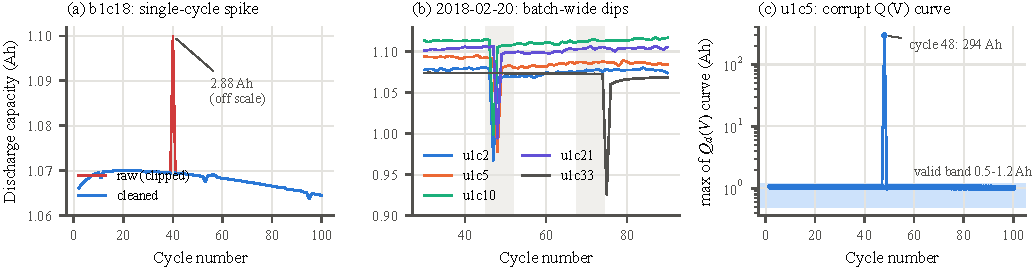
\includegraphics[width=\textwidth]{fig_clean_glitches}
  \caption{Capacity glitches. (a) A single-cycle spike to 2.88\,Ah in
  \texttt{b1c18}, removed by rule B3. (b) Dips at nearly the same cycles in
  many cells of the 2018-02-20 batch (shaded), pointing to test-wide
  interruptions rather than cell behaviour; \texttt{u1c33} also shows a
  small lasting step afterwards. (c) At a glitch cycle the interpolated
  discharge curve itself is corrupt, so curve validity is checked
  separately (rule B4).}
  \label{fig:glitches}
\end{figure*}

\begin{figure}[t]
  \centering
  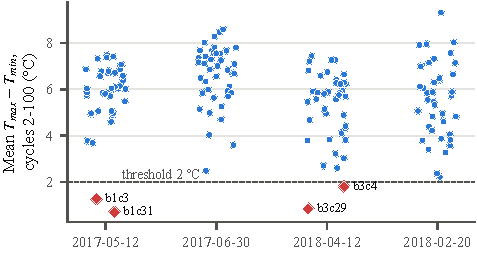
\includegraphics[width=\columnwidth]{fig_clean_temp}
  \caption{Average temperature swing within a cycle, for each cell. Healthy
  cells heat by about 6\,\textdegree C during the fast charge. Four cells
  stay below 2\,\textdegree C, which suggests a probe measuring chamber air
  (rule B6).}
  \label{fig:temp}
\end{figure}

\paragraph{Small lasting capacity steps}
After the test-wide interruptions in the 2018-02-20 batch, capacity
sometimes settles at a slightly different level (median $-1.6$\,mAh, range
$-11$ to $+5$\,mAh). We \emph{do not} correct these steps. They are
consistent with genuine recovery or loss of capacity during a rest, and we
cannot tell them apart from a measurement shift. They are small compared
with typical $|\dq|$ values (20--80\,mAh). They do, however, add noise to
the unseen batch, which we keep in mind when interpreting RQ5. For the same
reason, small gradual dips that recover over several cycles (e.g.\
\texttt{b1c5}, 5\,mAh at cycle 13) are left untouched.

\paragraph{How much data is affected}
In cycles 2--100 of the 163 cells used, rules B1--B5 mark 0.06\% of the
capacity values, 0.08\% of the charge-time values and 3.7\% of the IR
values as missing. The IR figure is almost entirely due to the six unseen
cells \texttt{u1c41}--\texttt{c46}, which have no IR record at all. Their IR
features will be filled with the training-set median, and this will be
reported. No cell needed a replacement curve at cycle 10 or 100.

\subsection{Verification against the original study}
The cleaned data was checked automatically (\texttt{src/checks.py}) against
Supplementary Table 9 of~\cite{severson2019}, which lists every cell with
its split, batch and cycle life:
\begin{itemize}
  \item \textbf{All 124 cells match exactly} on split, batch and cycle life.
  The range is 148--2237 cycles, as in the paper.
  \item The stored cycle life equals the first cycle with $Q_D<0.88$\,Ah in
  every cell. Where the test stopped just before crossing, as in
  \texttt{b1} and \texttt{b3} (final capacity 0.880--0.883\,Ah), it is
  $n_\text{cycles}+1$, which is the authors' own rule.
  \item Charging policies match for 2017-06-30 and 2018-04-12, once one
  naming alias is accepted (the paper's \texttt{4.36C(80\%)-4.36C} is
  recorded in the data as \texttt{4.8C(80\%)-4.8C-newstructure}). For
  2017-05-12, the paper's policy column is shifted from its ninth row on:
  it keeps the policies of the dropped cells. We therefore use each cell's
  own record in the data file.
\end{itemize}
Fig.~\ref{fig:overview} shows the cleaned capacity curves of all four sets.

\begin{figure*}[t]
  \centering
  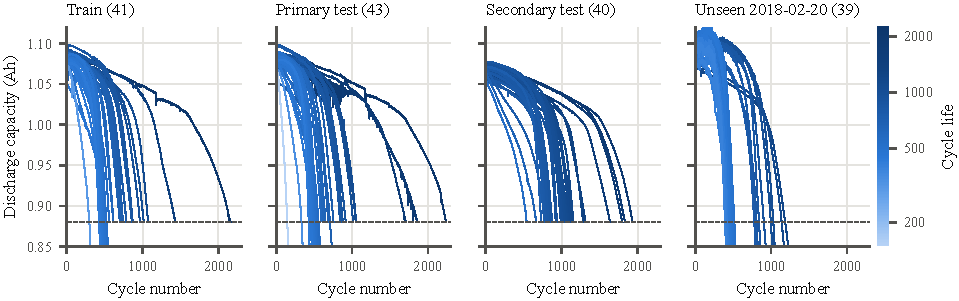
\includegraphics[width=\textwidth]{fig_dataset_overview}
  \caption{Cleaned discharge capacity of every cell in each set, coloured
  by cycle life. The dashed line is EOL (0.88\,Ah). The secondary test set
  and the unseen batch were run under different test procedures from the
  training data.}
  \label{fig:overview}
\end{figure*}

\subsection{Indexing convention}
The cached curves are stored by \emph{record}, while features are defined by
\emph{cycle number}. Record $j$ holds cycle number $j{+}1$ in every batch.
All code therefore accesses curves through one function,
\texttt{curve(cell, field, n)}, which looks up cycle number $n$ through the
summary's cycle array and applies rule B4. Record indices are never used
directly.

\subsection{Pipeline overview}
Fig.~\ref{fig:pipeline} summarises the pipeline. Every step is a script,
so the whole dataset can be rebuilt from the raw files with three commands
(\texttt{src.convert}, \texttt{src.clean}, \texttt{src.checks}).

\begin{figure}[t]
\centering
\begin{tikzpicture}[
  node distance=3.5mm,
  box/.style={draw, rounded corners=2pt, align=center, font=\footnotesize,
              minimum width=0.80\columnwidth, inner sep=3pt},
  arr/.style={-{Stealth[length=2mm]}, thick}]
  \node[box] (mat) {4 raw \texttt{.mat} batches (MATLAB v7.3 / HDF5), 2--3\,GB each};
  \node[box, below=of mat] (pkl) {\texttt{src/convert.py} $\rightarrow$ caches, about 90\,MB per batch\\
        (summaries + \texttt{Qdlin}/\texttt{Tdlin}/\texttt{dQdV}, first 160 records)};
  \node[box, below=of pkl] (clean) {\texttt{src/clean.py}: rules A1--A4 + B1--B10\\
        $\rightarrow$ \texttt{dataset.pkl} + \texttt{splits.json} (41/43/40 + 39)};
  \node[box, below=of clean] (chk) {\texttt{src/checks.py}: verify against SI Table 9 \checkmark};
  \node[box, below=of chk] (feat) {\texttt{src/features.py}: 20 features, cycles $\le 100$ $\rightarrow$ \texttt{features.csv}};
  \node[box, below=of feat] (model) {\texttt{src/reproduce.py}: paper's 3 models, reproduced (Sec.~\ref{sec:reproduction}) \checkmark};
  \node[box, below=of model] (f4) {\texttt{src/screen\_physics.py}, \texttt{src/p4\_*.py}: F4, model comparison \checkmark};
  \node[box, below=of f4, dashed] (next) {Unseen batch, interpretation \textit{(planned)}};
  \draw[arr] (mat) -- (pkl);
  \draw[arr] (pkl) -- (clean);
  \draw[arr] (clean) -- (chk);
  \draw[arr] (chk) -- (feat);
  \draw[arr] (feat) -- (model);
  \draw[arr] (model) -- (f4);
  \draw[arr] (f4) -- (next);
\end{tikzpicture}
\caption{Data pipeline. Solid boxes are complete; the dashed box is
planned.}
\label{fig:pipeline}
\end{figure}
